% !TEX spellcheck = de_DE
% !TeX root = Vorlesung.tex
%---------------------------------------------------------------------------------
\section[Blattentwurf]{Blattentwurf nach Betz}\label{sec:DES}
%---------------------------------------------------------------------------------
\miniframesoff
\begin{frame}<handout:0>[noframenumbering]{Inhalt}
\tableofcontents[currentsection]
\PutAt<1-|handout:0>[5cm]{(10cm,2cm)}{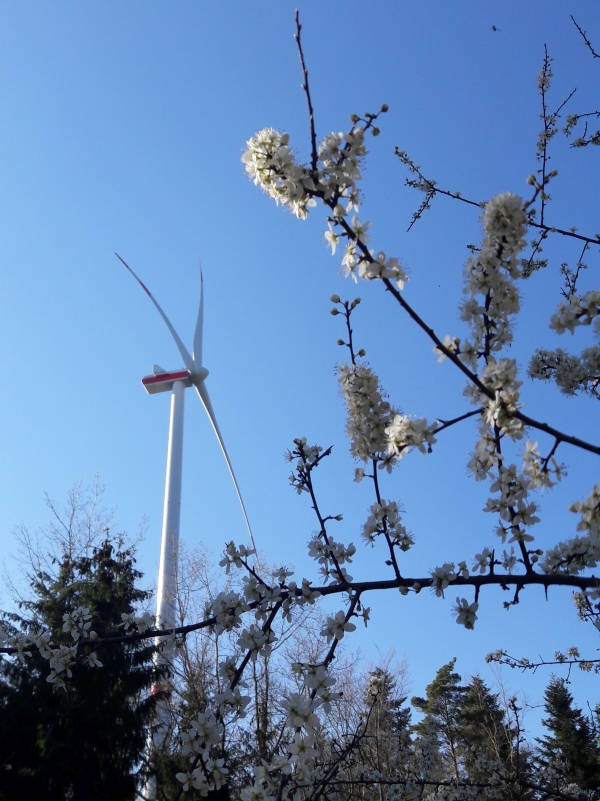
\includegraphics[width=4.0cm]{\StylePath/content/Fronrot2}} % graphic related to topic	
\end{frame}
\miniframeson
%---------------------------------------------------------------------------------
%%---------------------------------------------------------------------------------
\begin{frame}{Blattentwurf nach Betz - Konzept}
\begin{columns}	
	\column{10cm}
	\begin{block}<1->{Eingangsgrößen}
		\begin{itemize}
			\item Entwurfsschnelllaufzahl $\lambda_{\textnormal{D}}$
			\item Rotorradius $R$			
			\item Blattanzahl $z$
			\item Entwurfswerte von den Profilen 
				\begin{itemize}
					\item Anstellwinkel $\alpha_{\textnormal{A}}$ 
					\item Auftriebsbeiwert $c_{\textnormal{L}}$
				\end{itemize}			
		\end{itemize}		
	\end{block}	
	\begin{block}<1->{Ausgangsgrößen}
		\begin{itemize}
			\item Verlauf Verwindung $\beta(r)$ über dem Radius
			\item Verlauf Profiltiefe $c(r)$ über dem Radius	
		\end{itemize}		
	\end{block}		
	\column{4cm}
	\includegraphics<1->[width=4cm] {DES/MM92_Rotorblatt}
\end{columns} 	
\end{frame}
%%---------------------------------------------------------------------------------
\begin{frame}[t]{Blattentwurf nach Betz - Herleitung 1/7} 
\setlength{\abovedisplayskip}{0pt}
\setlength{\belowdisplayskip}{0pt}
\vspace*{-0.2cm} %compensate [t]
\begin{columns}[T]	
	\column{6cm}
	\begin{block}<1->{Anströmwinkel $\phi(r)$}
	\begin{align}		
	\tan{\left( \phi(r) \right)}&=\frac{v_2}{u(r)}=\frac{2 v_1}{3 \Omega r}\nonumber \\
	\lambda_{\textnormal{D}}& =\frac{\Omega R}{v_1} \label{equ:DES:lambda}
	\end{align}		
	\end{block}	
	\begin{block}<2->{Verwindung $\beta(r)$}
		\begin{align*}		
		\beta(r)   & = \phi(r)-\alpha_{\textnormal{A}}\\
		& = \arctan\left( \frac{2}{3} \frac{R}{r\lambda_{\textnormal{D}}}\right)-\alpha_{\textnormal{A}}
		\end{align*}		
	\end{block}	
	\column{8cm}
	\includegraphics<1->[width=8cm] {DES/Twist.pdf}
\end{columns} 
\begin{block}<3>{Blattentwurf nach Betz}
	Wir haben schon die erste Ausgangsgröße (Verwindung) abhängig nur von $R$, $\lambda_{\textnormal{D}}$, $\alpha_{\textnormal{A}}$! 
\end{block}		
\end{frame}
%%---------------------------------------------------------------------------------
\begin{frame}[t]{Blattentwurf nach Betz - Herleitung 2/7}
\vspace*{-0.2cm} %compensate [t]
\begin{columns}[T]	
	\column{6cm}
	\begin{block}<1->{Herleitung der Profiltiefe $c(r)$}
		\begin{enumerate}
			\item Herleitung Tangentialkräfte an jedem Blattelement
			\item Berechnung der mechanischen Leistung für jedes Blattelement unter Vernachlässigung des Widerstands
			\item Gleichsetzen der mechanischen mit der maximalen Leistung
			\item Verwendung des Geschwindigkeitsdreieck zur Herleitung der Profiltiefe
		\end{enumerate}	
	\end{block}	
	\column{8cm}
	\includegraphics<1->[width=8cm] {DES/Chord}
\end{columns} 		
\end{frame}
%---------------------------------------------------------------------------------
\begin{frame}[t]{Blattentwurf nach Betz - Herleitung Derivation 3/7} 
\setlength{\abovedisplayskip}{0pt}
\setlength{\belowdisplayskip}{0pt}
\vspace*{-0.2cm} %compensate [t]
\begin{columns}[T]	
	\column{6cm}
	\begin{block}<1->{Auftrieb $L$ und Widerstand $D$}
		\begin{align*}
		\textnormal{d}L   & = \frac{1}{2} \rho \left(c\textnormal{d}r\right) c_{\textnormal{L}}w^2\\
		\textnormal{d}D   & = \frac{1}{2} \rho \left(c\textnormal{d}r\right) c_{\textnormal{D}}w^2
		\end{align*}
		\begin{tabular}{ll}
			$\textnormal{d}r$ 		&	Profilbreite des Elements bei $r$ 
		\end{tabular}	
	\end{block}
	\begin{block}<2->{Tangentialkraft $U$ und \\ Schubkraft $T$}
		\begin{align}
		\textnormal{d}U   	& = \textnormal{d}U_L - \textnormal{d}U_D 				\nonumber\\
		& = \sin(\phi)\textnormal{d}L-\cos(\phi)\textnormal{d}D \label{equ:DES:U}\\
		\textnormal{d}T   	& = \textnormal{d}T_L+\textnormal{d}T_D 				\nonumber\\
		& = \cos(\phi)\textnormal{d}L+\sin(\phi)\textnormal{d}D \nonumber
		\end{align}	
	\end{block}
	\column{8cm}
	\only<1|handout:0>{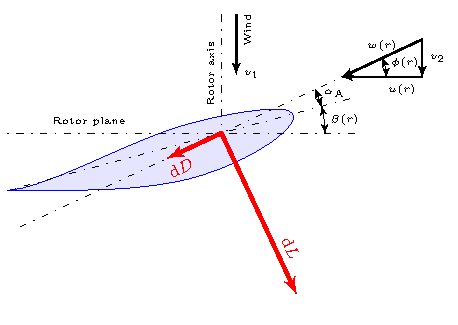
\includegraphics[width=8cm] {DES/Triangle1.pdf}}%
	\only<2|handout:0>{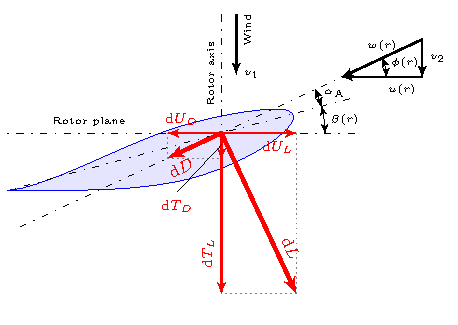
\includegraphics[width=8cm] {DES/Triangle2.pdf}}%
	\only<3|handout:1>{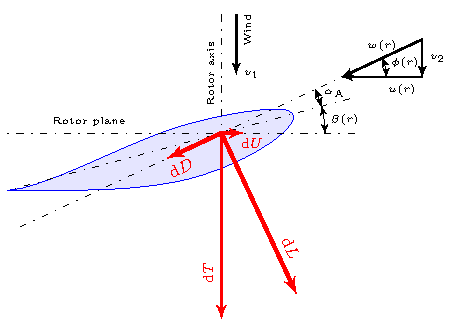
\includegraphics[width=8cm] {DES/Triangle3.pdf}}%
\end{columns}	
\end{frame}
%%---------------------------------------------------------------------------------
\begin{frame}{Blattentwurf nach Betz - Herleitung 4/7} 
\setlength{\abovedisplayskip}{0pt}
\setlength{\belowdisplayskip}{0pt}
\begin{columns}	
	\column{9cm}
	\begin{block}<1->{Mechanische Leistung für jeden Ringabschnitt}
		\begin{align}
		\textnormal{d}P_{\textnormal{mech}} 	
		& = z \textnormal{d}U r \Omega \quad\textnormal{mit}\quad c_{\textnormal{D}} \ll c_{\textnormal{L}} \quad\textnormal{und}\quad (\ref{equ:DES:U}) \nonumber\\
		& = z   \sin(\phi) \frac{1}{2} \rho \left(c\textnormal{d}r\right)w^2 c_{\textnormal{L}} r \Omega \label{equ:DES:dP}
		\end{align}
		\begin{tabular}{ll}
			$z$ 		& Blattanzahl
		\end{tabular}			
	\end{block}	
	\begin{block}<2->{Maximale der Kreisfläche entnehmbare Leistung}
		\begin{align*}
		P_{\textnormal{Betz}}   & = \frac{16}{27} \frac{1}{2}\rho  Av_1^3
		\end{align*}		
	\end{block}	
	\begin{block}<3->{Maximale Leistung für Ringabschnitt $\textnormal{d}A=2\pi r \textnormal{d}r$}
		\begin{align}
		\textnormal{d}P_{\textnormal{Betz}}   & = \frac{16}{27} \frac{1}{2}\rho (2\pi r \textnormal{d}r) v_1^3\label{equ:DES:dPBetz}
		\end{align}		
	\end{block}	
	\column{5cm}
	\includegraphics<1->[width=5cm] {DES/RingSection}\\% ersetzen durch Tikz aus IWTA#06
	\flushright\tiny\textcolor{gray}{\cite{Gasch2016}}
\end{columns} 	
\end{frame}
%%---------------------------------------------------------------------------------
\begin{frame}{Blattentwurf nach Betz - Herleitung 5/7} 
\begin{block}<1->{}
	Gleichung (\ref{equ:DES:dPBetz}) mit (\ref{equ:DES:dP}) gleichsetzen ergibt
	\begin{align*}
	\frac{16}{27} \frac{1}{2}\rho \left( 2\pi r \textnormal{d}r \right) v_1^3 & = z \sin{(\phi)} \frac{1}{2} \rho ( c \textnormal{d} r ) w^2 c_{\textnormal{L}} r \Omega 
	\end{align*}		
\end{block}		
\begin{block}<2->{}
	Vereinfachen ergibt
	\begin{align*}			
	\frac{16}{27} \frac{1}{\cancel{2}} \cancel{\rho} \left( 2\pi \cancel{r} \cancel{\textnormal{d}r} \right) v_1^3 & = z \sin{(\phi)} \frac{1}{\cancel{2}} \cancel{\rho} ( c \cancel{\textnormal{d}r} ) w^2 c_{\textnormal{L}}\cancel{r} \Omega \\
	\frac{16}{27}  \left( 2\pi \right) v_1^3 & = z \sin{(\phi)}  c   w^2 c_{\textnormal{L}} \Omega
	\end{align*}			
\end{block}	
\begin{block}<3->{}
	Umstellen ergibt (Profiltiefe abhängig von $v_1$, $w$, $\Omega$, $\phi$, also nicht nur von Eingangsgrößen!)
	\begin{align}			
	c   & = \frac{1}{z} \frac{16}{27} \frac{2\pi}{c_{\textnormal{L}}} \frac{v_1^3}{\Omega w^2 \sin(\phi)} \label{equ:DES:c}
	\end{align}			
\end{block}	
\end{frame}
%%---------------------------------------------------------------------------------
%%---------------------------------------------------------------------------------
\begin{frame}[t]{Blattentwurf nach Betz - Herleitung 6/7} 
\setlength{\abovedisplayskip}{0pt}
\setlength{\belowdisplayskip}{0pt}
\vspace*{-0.2cm} %compensate [t]
\begin{columns}[T]	
	\column{6cm}	
	\begin{block}<1->{Zu ersetzen}
		\begin{align*}			
		\frac{v_1^3}{\Omega w^2 \sin(\phi)}
		\end{align*}			
	\end{block}	
	\begin{block}<2->{Geschwindigkeitsdreieck}
		\begin{align}	
		\Omega & = \frac{\lambda_{\textnormal{D}} v_1}{R}\label{equ:DES:Omega}\\
		w \sin{(\phi)}& = \frac{2}{3} v_1\label{equ:DES:sin}
		\end{align}	
	\end{block}	
	\column{8cm}
	\includegraphics<1->[width=8cm] {DES/Twist.pdf}
\end{columns}
\vspace*{-.5cm} 	
\begin{block}<3->{}	
	\begin{align}
	w^2 &= \left( \frac{2}{3}v_1 \right)^2 + \left( \Omega r \right)^2 = \frac{4}{9}v_1^2+ \left( \frac{\lambda_{\textnormal{D}}v_1}{R} \right)^2 r^2 \quad \Rightarrow \quad w=v_1 \sqrt{\left( \frac{r}{R}\lambda_{\textnormal{D}} \right)^2 + \frac{4}{9}}\label{equ:DES:w}
	\end{align}
\end{block}	
\end{frame}
%%---------------------------------------------------------------------------------
\begin{frame}{Blattentwurf nach Betz - Herleitung 7/7} 
\setlength{\abovedisplayskip}{0pt}
\setlength{\belowdisplayskip}{0pt}
\begin{block}<1->{}
	Einsetzen von (\ref{equ:DES:Omega},\ref{equ:DES:sin},\ref{equ:DES:w})  in (\ref{equ:DES:c}) ergibt:
	\begin{align*}
	c(r) 	&  = \frac{1}{z} \frac{16}{27} \frac{2\pi}{c_{\textnormal{L}}} \frac{v_1^3}{\Omega w^2 \sin(\phi)}\\
	&  = \frac{1}{z} \frac{16}{27} \frac{2\pi}{c_{\textnormal{L}}} \frac{v_1^3}{\frac{\lambda_{\textnormal{D}} v_1}{R} \frac{2}{3}v_1 v_1 \sqrt{\left( \frac{r}{R}\lambda_{\textnormal{D}} \right)^2 + \frac{4}{9}}}
	\end{align*}
\end{block}
\begin{block}<2->{Verlauf Profiltiefe $c(r)$}
	\begin{align*}
	c(r) & = \frac{1}{z} \frac{8}{9} \frac{2\pi R}{c_{\textnormal{L}}} \frac{1}{ \lambda_{\textnormal{D}} \sqrt{\left(\lambda_{\textnormal{D}}\frac{r}{R} \right)^2+\frac{4}{9}}} 
	\end{align*}
\end{block}
\begin{block}<3>{Blattentwurf nach Betz}
	Wir haben nun die 2. Ausgangsgröße (Profiltiefe) abhängig nur von $z$, $R$, $\lambda_{\textnormal{D}}$, $c_{\textnormal{L}}$! 
\end{block}	
\end{frame}
%%---------------------------------------------------------------------------------
\begin{frame}{Einfluss der Entwurfsschnelllaufzahl $\lambda_{\textnormal{D}}$} 
\begin{columns}
    \column{7cm}
    \includegraphics<1->[width=7cm] {DES/Gasch2016_Abb5.17.pdf}\\
    \tiny\textcolor{gray}{\cite{Gasch2016}}
    \column{7cm}
	\includegraphics<1->[width=7cm] {DES/Hau2014_Fig5.47.jpg}\\
	\flushright\tiny\textcolor{gray}{\cite{Hau2014}}
\end{columns}
\end{frame}
%---------------------------------------------------------------------------------
\begin{frame}{Flächenfüllungsgrad} 
\centering
\includegraphics<1->[height=7cm] {DES/Gasch2016_Abb5.15.jpg}\\
\tiny\textcolor{gray}{\cite{Gasch2016}}
\end{frame}
%%---------------------------------------------------------------------------------
\begin{frame}{Anmerkung: Reale Anlagen erreichen nicht das Betz Limit} 
\centering
	\begin{block}<1->{}	
	\begin{itemize}
		\item maximaler Leistungsbeiwert nach Betz $16/27 \approx \SI{59}{\percent}$		
		\item realer Leistungsbeiwert normalerweise um die $\SI{43}{\percent}-\SI{48}{\percent}$
		\item Enercon E66 mit E4-Blade erreicht $\SI{52}{\percent}$ 
	\end{itemize}	
	\end{block}
\includegraphics<1->[width=5.5cm] {DES/Enercon1}
\includegraphics<1->[width=5.5cm] {DES/Enercon2}
\tiny\textcolor{gray}{[Enercon]}
\end{frame}
%---------------------------------------------------------------------------------
\begin{frame}{Einige Eindrücke von der ursprünglichen Arbeit von Betz 1/3} 
\begin{columns}	
	\column{7cm}
		\centering
		\includegraphics<1->[height=7.5cm] {DES/Betz1926_Frontpage}{\tiny\textcolor{gray}{\cite{Betz1926}}}
	\column{7cm}
		\centering
		\includegraphics<2->[height=7.5cm] {DES/Betz1926_Abb7}
\end{columns} 
\end{frame}
%---------------------------------------------------------------------------------
\begin{frame}{Einige Eindrücke von der ursprünglichen Arbeit von Betz 2/3} 
	\centering
	\includegraphics<1->[height=7.5cm] {DES/Betz1926_Page12and13}
	{\tiny\textcolor{gray}{\cite{Betz1926}}}
\end{frame}
%---------------------------------------------------------------------------------
\begin{frame}{Einige Eindrücke von der ursprünglichen Arbeit von Betz 3/3} 
\centering
\includegraphics<1->[height=7.5cm] {DES/Betz1926_Page24and25}
{\tiny\textcolor{gray}{\cite{Betz1926}}}
\end{frame}
%---------------------------------------------------------------------------------
\begin{frame}{Ausblick: Reale Rotorblätter sehen anders aus!} 
\centering
\includegraphics<1->[width=6.5cm] {DES/Gasch2012_Fig3.9.jpg}{\tiny\textcolor{gray}{\cite{Gasch2016}}}
\includegraphics<1->[width=6.5cm] {DES/MM92_blade.jpg}
\end{frame}
%---------------------------------------------------------------------------------
\begin{frame}{Ausblick: Blattentwurf nach Schmitz} 
\begin{columns}	
	\column{7cm}
	\begin{block}<1->{Betrachtung realer Effekte}	
		\begin{itemize}
			\item Verlust durch Drall
			\item Profilwiderstand
			\item endliche Blattanzahl
		\end{itemize}	
	\end{block}
	\includegraphics<1->[height=4.5cm] {DES/Hau2014_Fig5.6.jpg}\\
	\flushright\tiny\textcolor{gray}{\cite{Hau2014}}	
	\column{7cm}
	\begin{block}<2->{Vergleich der Profiltiefe}	
		\begin{itemize}
			\item ähnlich für große $\lambda_{\textnormal{D}}$ und nahe der Spitze
			\item unterschiedlich für kleine $\lambda_{\textnormal{D}}$ und Nahe der Nabe
		\end{itemize}	
	\end{block}%
	\includegraphics<2->[width=7.0cm] {DES/Gasch2012_Fig5.22}%
	\visible<2->{\flushright{\tiny\textcolor{gray}{\cite{Gasch2016}}}}%
\end{columns} 
\end{frame}
%%---------------------------------------------------------------------------------